\documentclass[12pt]{article}
% REVISION NOTES %%%%%%%%%%%%%%%%%%%%%%%%%%%%%%%%%%%%%%%%%%%%
% 2008-0814 Location, Date, Time
% 2008-0814 fixed citations -- added bibliography.
%
%
\usepackage{geometry}                
\geometry{letterpaper}                   
%\geometry{landscape}                
\usepackage[parfill]{parskip}    
\usepackage{daves,fancyhdr,natbib,graphicx,dcolumn,amsmath,lastpage,url}
\usepackage{amsmath,amssymb,epstopdf,longtable}
\usepackage[final]{pdfpages}
\DeclareGraphicsRule{.tif}{png}{.png}{`convert #1 `dirname #1`/`basename #1 .tif`.png}
\pagestyle{fancy}
\lhead{CE 3305 -- Fluid Mechanics -- SPRING 2024}
\rhead{Name:\_\_\_\_\_\_\_\_\_\_\_\_\_\_\_\_\_\_\_\_\_\_\_\_\_\_\_\_\_\_\_\_\_\_\_\_\_\_\_\_\_\_\_\_}
\lfoot{CE 3305 -- Cleveland}
\cfoot{Page \thepage\ of \pageref{LastPage}}
\rfoot{REVISED: ~4 FEB 2024}
\renewcommand\headrulewidth{0pt}
%%%%%%%%%%%%%%%%%%%%%%%%%%%%%%%%%%%%%%%%%%%%%%%%%%%%%%%
\begin{document}
\section*{\center{ {CE 3305 -- Fluid Mechanics Exam 2 Extra Credit} } }
\section*{Problem}
A small piece of volcanic ejecta from Amboy Crater is at the front of
the classroom

\begin{figure}[htbp] %  figure placement: here, top, bottom, or page
   \centering
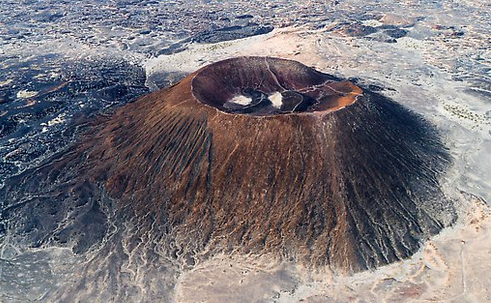
\includegraphics[width=2in]{amboy.png}
\end{figure}

The mass of the object is 23.93 grams. The porosity of typical pumice is
\(\eta = 64–85\%\) by volume
\url{https://en.wikipedia.org/wiki/Pumice}

The ellipsoid method to approximate volume uses 3 measurements
\(A\),\(B\), and \(C\), called semi-axes.

\begin{figure}[htbp] %  figure placement: here, top, bottom, or page
\centering
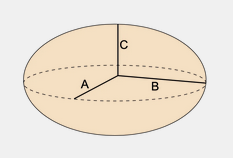
\includegraphics[width=2in]{ellipsoid.png}
\end{figure}

\(V = \frac{4}{3} * \pi * A * B * C\)

The porosity of typical pumice is \(\eta = 64–85\%\) by volume. The porosity can
be used to approximate the solids volume from the expression:

\(V_{total} \cdot (1-\eta) \approx V_{solids}\)

Determine: 
\begin{enumerate}
\item An estimate of the volume of the irregular shaped object (in milliliters). 
\item An estimate of the solids volume, based on a porosity of \(64\%\) 
\item Will it float?

\end{enumerate}


    
    
    
\end{document}
